\documentclass[a4paper,11pt]{article}

\usepackage[utf8]{inputenc}
\usepackage[T1]{fontenc}
\usepackage[french]{babel}
\usepackage{lmodern}
\usepackage{microtype}
\usepackage{graphicx}
\usepackage{hyperref}
\usepackage{xcolor}
\usepackage{tcolorbox}
\usepackage{enumitem}
\usepackage{geometry}
\usepackage{fancyhdr}
\usepackage[table]{xcolor}
\usepackage{booktabs}
\usepackage{array}
\usepackage{tabularx}
\usepackage{listings}
\usepackage{fancyvrb}
\usepackage{multicol}

\geometry{margin=2cm, top=2.5cm, bottom=2.5cm}
\setlength{\headheight}{14pt}

\definecolor{titlecolor}{RGB}{0, 90, 160}
\definecolor{sectitlecolor}{RGB}{5, 100, 175}
\definecolor{subsectitlecolor}{RGB}{10, 110, 190}
\definecolor{definitionbg}{RGB}{240, 248, 255}
\definecolor{examplebg}{RGB}{245, 255, 245}
\definecolor{warningbg}{RGB}{255, 245, 245}
\definecolor{benefitbg}{RGB}{255, 253, 235}
\definecolor{codecolor}{RGB}{240, 240, 240}
\definecolor{codekeyword}{RGB}{0, 0, 128}
\definecolor{codestring}{RGB}{163, 21, 21}
\definecolor{codecomment}{RGB}{0, 128, 0}
\definecolor{todobg}{RGB}{255, 235, 235}
\definecolor{collabg}{RGB}{245, 240, 255}

\lstset{
  basicstyle=\ttfamily\footnotesize,
  backgroundcolor=\color{codecolor},
  keywordstyle=\color{codekeyword}\bfseries,
  stringstyle=\color{codestring},
  commentstyle=\color{codecomment}\itshape,
  breaklines=true,
  showstringspaces=false,
  frame=single,
  tabsize=2,
  captionpos=b
}

\pagestyle{fancy}
\fancyhf{}
\fancyhead[L]{\textit{Lab 3 --- Le monolithe modulaire}}
\fancyhead[R]{\textit{Architectures Logicielles}}
\fancyfoot[C]{\thepage}
\fancyfoot[L]{\textit{Dr. El Hadji Bassirou TOURE}}
\fancyfoot[R]{\textit{DMI/FST/UCAD}}
\renewcommand{\headrulewidth}{0.4pt}
\renewcommand{\footrulewidth}{0.4pt}

\newtcolorbox{concept}{
  colback=definitionbg, colframe=sectitlecolor,
  title=Concept fondamental, fonttitle=\bfseries
}
\newtcolorbox{intuition}{
  colback=examplebg, colframe=green!75!black,
  title=Intuition, fonttitle=\bfseries
}
\newtcolorbox{exemple}{
  colback=orange!5!white, colframe=orange!75!black,
  title=Exemple, fonttitle=\bfseries, fontupper=\footnotesize
}
\newtcolorbox{pointcle}{
  colback=benefitbg, colframe=orange!70!black,
  title=Point cle a retenir, fonttitle=\bfseries
}
\newtcolorbox{warningbox}{
  colback=warningbg, colframe=red!70!black,
  title=Point d'attention, fonttitle=\bfseries
}
\newtcolorbox{benefitbox}{
  colback=benefitbg, colframe=green!70!black,
  title=Benefice, fonttitle=\bfseries
}
\newtcolorbox{todobox}{
  colback=todobg, colframe=red!60!black,
  title=Tache a realiser, fonttitle=\bfseries\scriptsize, fontupper=\small
}
\newtcolorbox{collabox}{
  colback=collabg, colframe=violet!70!black,
  title=Qui pilote cette section ?, fonttitle=\bfseries\scriptsize, fontupper=\small
}
\newtcolorbox{tagbox}{
  colback=yellow!15, colframe=yellow!50!black,
  title=Jalon Git, fonttitle=\bfseries\scriptsize, fontupper=\small
}

\lstset{
  basicstyle=\tiny\ttfamily,
  keywordstyle=\tiny\ttfamily\bfseries\color{codekeyword},
  commentstyle=\tiny\ttfamily\itshape\color{codecomment},
  stringstyle=\tiny\ttfamily\color{codestring}
}

\usepackage[explicit]{titlesec}
\titleformat{\section}
  {\Large\bfseries\color{titlecolor}}{\thesection}{0.5em}{#1}
\titleformat{\subsection}
  {\large\bfseries\color{sectitlecolor}}{\thesubsection}{0.5em}{#1}
\titleformat{\subsubsection}
  {\normalsize\bfseries\color{subsectitlecolor}}{\thesubsubsection}{0.5em}{#1}

\title{\textcolor{titlecolor}{\Huge\textbf{Lab 4 --- L'extraction}}\\[0.5em]
       \textcolor{sectitlecolor}{\LARGE Un module quitte le monolithe : microservice FastAPI, compose et carte}}
\author{Dr. El Hadji Bassirou TOURE\\
        Département de Mathématiques et Informatique\\
        Faculté des Sciences et Techniques\\
        Université Cheikh Anta Diop}
\date{Année universitaire 2026--2027}

\begin{document}

\maketitle
\thispagestyle{empty}

\begin{abstract}
\noindent La direction de SénResto veut faire évoluer le calcul d'itinéraires
avec l'écosystème géospatial de Python, et déployer ces évolutions sans
redéployer le reste. Ce lab répond par l'\textbf{extraction} : le module
\texttt{livraison} quitte le monolithe et devient \textbf{livraison-service},
un microservice \textbf{FastAPI}, selon le pattern \textbf{Strangler Fig} ---
le nouveau pousse autour de l'ancien, l'application fonctionne à chaque
instant. Côté monolithe, \texttt{AssignationLivreurs} garde exactement la
même API mais devient une \emph{façade} qui traverse le réseau ---
\texttt{commandes} ne remarquera rien. \textbf{docker compose} orchestre les
quatre conteneurs, une \textbf{carte Leaflet de Dakar} suit le livreur en
temps réel, et la séance se clôt sur une expérience fondatrice : nous
\textbf{tuerons le service} pour regarder mourir la confirmation de commande
--- le cliffhanger du Lab 5.
\end{abstract}

\begin{benefitbox}
À l'issue de ce lab, vous saurez :
\begin{itemize}[nosep]
  \item justifier (ou refuser) une extraction : technologie, déploiement,
        dimensionnement --- et défendre des non-décisions ;
  \item extraire un module en \textbf{Strangler Fig}, sans interruption de
        service, grâce aux frontières du modulith ;
  \item écrire un microservice \textbf{FastAPI} et le faire dialoguer avec
        Spring via \textbf{RestClient} (timeouts, traduction d'erreurs) ;
  \item orchestrer un système multi-conteneurs avec \textbf{docker compose},
        et brancher une carte \textbf{Leaflet} sans clé API.
\end{itemize}
\end{benefitbox}

\begin{warningbox}
\textbf{Prérequis avant la séance :}
\begin{itemize}[nosep]
  \item votre dépôt au tag \texttt{lab4-depart} (= \texttt{lab3-final}) ;
        \texttt{./mvnw clean test} vert : \textbf{10 juges} ;
  \item \textbf{Python 3.12+} installé (\texttt{python3 --version}) ;
        Docker Desktop fonctionnel ;
  \item connexion internet (pip : fastapi, uvicorn ; npm : react-leaflet).
\end{itemize}
\end{warningbox}

\tableofcontents
\newpage

% =====================================================================
\section{Le constat : une bonne raison, un bon candidat}
% =====================================================================

\begin{intuition}
On ne déménage pas parce que déménager est à la mode : on déménage parce
que le nouveau logement offre ce que l'ancien ne peut pas offrir. Un
microservice, c'est pareil --- et la première tâche de l'architecte est de
vérifier que la raison est réelle et que le candidat est le bon.
\end{intuition}

\subsection{Exercice (10 minutes, en groupe)}

Pour chacun des sept modules, répondez : une autre technologie lui
serait-elle utile ? Un déploiement indépendant ? Un dimensionnement
indépendant ? Ses données sont-elles partagées ? Concluez : quel est LE
candidat --- et pourquoi les six autres ne le sont pas. Gardez vos notes :
c'est la matière première de l'ADR n\up{o}4, le premier qui devra défendre
des \emph{non-décisions}.

\begin{pointcle}
\texttt{livraison} coche toutes les cases : frontière nette (Lab 3), API
étroite (\texttt{assigner}, \texttt{liberer}, \texttt{tous}), données
propres (les livreurs), raison technologique (l'écosystème géo de Python)
et raison de déploiement (évolutions fréquentes demandées). C'est
l'extraction \emph{la moins chère} avec le bénéfice \emph{le plus clair}.
\end{pointcle}

\begin{concept}
\textbf{Strangler Fig (Fowler).} Plutôt que le « big bang » (tout
réécrire, tout basculer, prier), le nouveau système \textbf{pousse autour
de l'ancien} : on construit le service à côté, on fait basculer la façade,
l'ancien code meurt quand plus rien ne l'appelle. À chaque commit,
l'application fonctionne. Notre monolithe modulaire rend l'opération
presque chirurgicale : la frontière et l'API existent déjà.
\end{concept}

\begin{figure}[h]
\centering
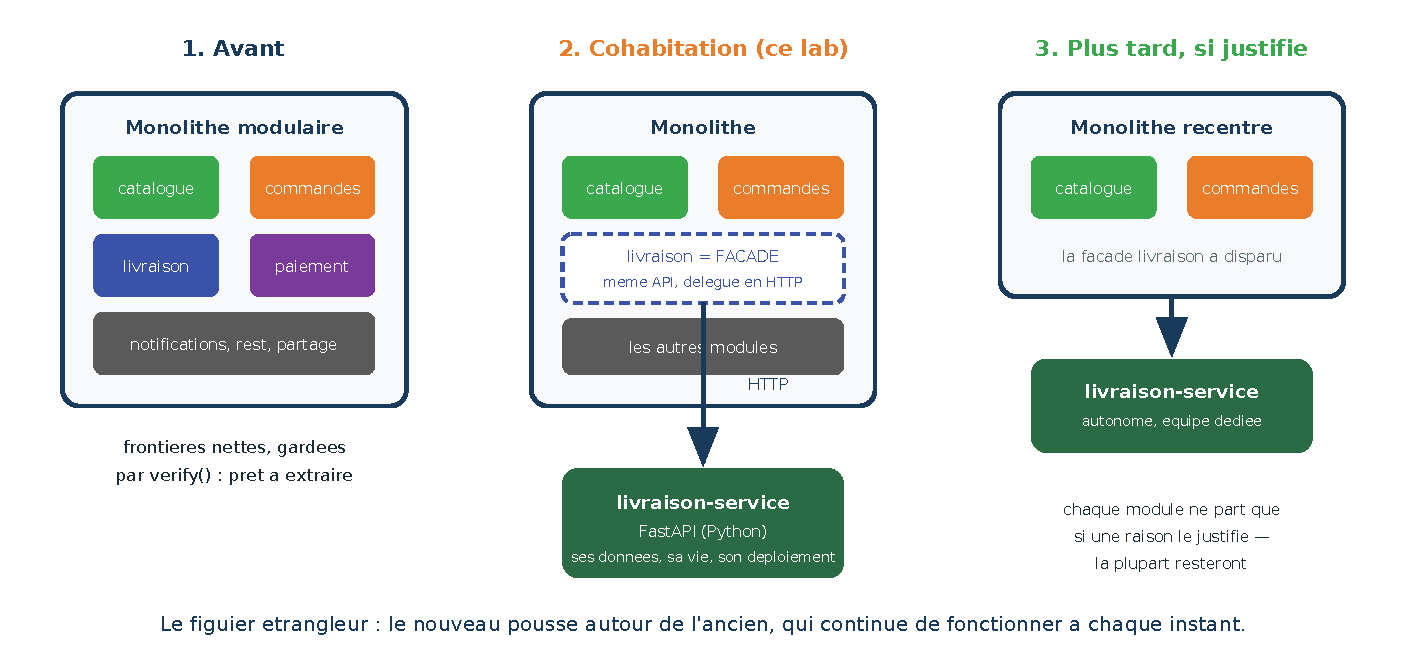
\includegraphics[width=0.88\textwidth]{figs/figJ_strangler.pdf}
\caption{Le figuier étrangleur : trois phases, zéro interruption.}
\end{figure}

% =====================================================================
\section{Etape 1 --- Le service Python nait}
% =====================================================================

\begin{collabox}
\textbf{L'Appariteur} pilote le nouveau service --- c'est son jour de
gloire. \textbf{Le Notaire} relit le contrat HTTP contre l'API du module
(mêmes règles, mêmes messages). \textbf{Les autres} préparent l'étape 2.
\end{collabox}

À la racine du dépôt (à côté de \texttt{backend/} et \texttt{frontend/}),
créez \texttt{livraison-service/} :

\begin{lstlisting}[language=bash]
livraison-service/
|-- main.py             # l'application FastAPI complete
|-- requirements.txt    # fastapi + uvicorn
\-- Dockerfile          # pour l'etape finale
\end{lstlisting}

\subsection{Le contrat d'abord}

Le service traduit l'API du module en HTTP --- vocabulaire et messages
\textbf{strictement identiques} :

\begin{lstlisting}[language=bash]
POST   /assignations    {"quartier": "Medina",
                         "restaurant_quartier": "Ouakam"}
       -> 200 {"livreur_id": 1, "livreur_nom": "...", "eta_minutes": 43}
       -> 409 {"erreur": "Aucun livreur disponible pour le moment, ..."}
DELETE /assignations/{livreur_id}     # liberer
GET    /livreurs                      # liste complete
GET    /livreurs/{id}/position        # position simulee (pour la carte)
\end{lstlisting}

\subsection{main.py : le service complet}

Le c\oe ur du service --- remarquez que \texttt{QuartiersDakar} et le
calcul d'ETA \textbf{déménagent en Python} : le service possède désormais
ce savoir, et ses données livreurs vivent en mémoire chez lui
(\emph{database per service}, version simple) :

\begin{lstlisting}[language=python]
from fastapi import FastAPI, HTTPException
from fastapi.middleware.cors import CORSMiddleware
from pydantic import BaseModel
import math, time

app = FastAPI(title="SenResto - Service Livraison")
app.add_middleware(CORSMiddleware, allow_origins=["*"],
                   allow_methods=["*"], allow_headers=["*"])

QUARTIERS = {  # l'ex-QuartiersDakar, desormais propriete du service
    "Plateau":     {"frais": 1000, "lat": 14.667, "lng": -17.436},
    "Medina":      {"frais": 1000, "lat": 14.677, "lng": -17.451},
    # ... les 7 quartiers, memes valeurs qu'au Lab 3 ...
}

LIVREURS = {   # ses donnees, chez lui (memes valeurs que data.sql)
    1: {"nom": "Ibrahima Ndiaye", "telephone": "771112233",
        "lat": 14.690, "lng": -17.446, "disponible": True},
    2: {"nom": "Cheikh Sarr", "telephone": "772223344",
        "lat": 14.710, "lng": -17.470, "disponible": True},
}
COURSES = {}   # livreur_id -> details de la course en cours (pour la carte)

class DemandeAssignation(BaseModel):
    quartier: str                          # celui du client
    restaurant_quartier: str | None = None # celui du restaurant

def distance_km(lat1, lng1, lat2, lng2):
    d_lat, d_lng = math.radians(lat2 - lat1), math.radians(lng2 - lng1)
    a = (math.sin(d_lat / 2) ** 2 + math.cos(math.radians(lat1))
         * math.cos(math.radians(lat2)) * math.sin(d_lng / 2) ** 2)
    return 6371.0 * 2 * math.atan2(math.sqrt(a), math.sqrt(1 - a))

@app.post("/assignations")
def assigner(demande: DemandeAssignation):
    cible = QUARTIERS.get(demande.quartier)
    if cible is None:
        raise HTTPException(400, detail="Quartier non livrable")
    candidats = [i for i, l in LIVREURS.items() if l["disponible"]]
    if not candidats:
        raise HTTPException(409, detail="Aucun livreur disponible "
                            "pour le moment, reessayez plus tard")
    livreur_id = min(candidats)          # meme regle : le premier par id
    livreur = LIVREURS[livreur_id]
    # Le trajet REEL : livreur -> restaurant (recuperer le plat) -> client.
    resto = QUARTIERS.get(demande.restaurant_quartier or "")
    points = [(livreur["lat"], livreur["lng"])]
    if resto is not None:
        points.append((resto["lat"], resto["lng"]))
    points.append((cible["lat"], cible["lng"]))
    d = sum(distance_km(*points[i], *points[i + 1])
            for i in range(len(points) - 1))
    eta = math.ceil(d / 18.0 * 60.0) + 10
    livreur["disponible"] = False
    COURSES[livreur_id] = {"points": points,
                           "debut": time.time(), "duree_s": eta * 60}
    return {"livreur_id": livreur_id, "livreur_nom": livreur["nom"],
            "eta_minutes": eta}
\end{lstlisting}

Complétez sur le même modèle : \texttt{DELETE /assignations/\{id\}} (le
livreur redevient disponible, sa course s'efface), \texttt{GET /livreurs},
et la position simulée --- une interpolation \emph{par morceaux} le long des jambes du
trajet (livreur $\to$ restaurant $\to$ client), au prorata de la distance
--- le squelette complet est fourni dans le zip :

\begin{lstlisting}[language=python]
@app.get("/livreurs/{livreur_id}/position")
def position(livreur_id: int):
    course = COURSES.get(livreur_id)
    # ... 404 si livreur inconnu ; point d'attache si pas en course ...
    avancement = min(1.0, (time.time() - course["debut"]) / course["duree_s"])
    # interpolation PAR MORCEAUX sur course["points"], au prorata
    # de la distance parcourue (voir le corrige) :
    #   d_parcourue = avancement * d_totale, puis on avance de jambe
    #   en jambe jusqu'a trouver celle qui contient d_parcourue.
    return {"latitude": lat, "longitude": lng, "avancement": round(avancement, 3)}
\end{lstlisting}

\subsection{Premier vol, au curl}

\begin{lstlisting}[language=bash]
cd livraison-service
python3 -m venv .venv && source .venv/bin/activate
pip install fastapi uvicorn
uvicorn main:app --port 8001 --reload

# Dans un second terminal :
curl -s -X POST localhost:8001/assignations \
     -H "Content-Type: application/json" -d '{"quartier": "Medina"}'
# {"livreur_id":1,"livreur_nom":"Ibrahima Ndiaye","eta_minutes":16}
curl -s localhost:8001/livreurs/1/position     # elle bouge !
curl -s -X POST ... une 3e assignation -> 409  # plus de livreur
\end{lstlisting}

\begin{tagbox}
Le service répond au curl sur les quatre endpoints, le 409 au bon moment :
\begin{center}
\texttt{git tag lab4-etape1 \&\& git push origin lab4-etape1}
\end{center}
\end{tagbox}

% =====================================================================
\section{Etape 2 --- La facade : le monolithe traverse le reseau}
% =====================================================================

\begin{collabox}
\textbf{Le Notaire} pilote l'adaptateur HTTP. \textbf{L'Huissier} pilote
les profils Spring. \textbf{Le Doyen} vérifie l'invariant sacré : pas une
ligne modifiée dans \texttt{commandes}.
\end{collabox}

\subsection{Le Strangler en action : deux implementations cohabitent}

C'est ici que le pattern prend chair. \texttt{AssignationLivreurs} devient
une \textbf{interface} (l'API publique ne change pas d'une signature), et
\emph{deux} implémentations vivent côte à côte dans \texttt{interne/} :

\begin{lstlisting}[language=java]
// livraison/AssignationLivreurs.java  -- devient une interface
public interface AssignationLivreurs {
    Optional<Assignation> assigner(String quartier);
    void liberer(long livreurId);
    List<Map<String, Object>> tous();
}
\end{lstlisting}

\begin{lstlisting}[language=java]
// livraison/interne/AssignationLocale.java -- l'ANCIENNE implementation
// (l'ex-classe du Lab 3, renommee ; JDBC + CalculateurEta inchanges)
@Profile("!distribue")
@Component
class AssignationLocale implements AssignationLivreurs { /* ... */ }
\end{lstlisting}

\begin{lstlisting}[language=java]
// livraison/interne/AdaptateurLivraisonHttp.java -- la NOUVELLE
@Profile("distribue")
@Component
class AdaptateurLivraisonHttp implements AssignationLivreurs {

    private final RestClient client;

    AdaptateurLivraisonHttp(@Value("${livraison.url}") String url) {
        this.client = RestClient.builder()
                .baseUrl(url)
                .requestFactory(usineAvecTimeouts())   // 2 s connexion, 3 s lecture
                .build();
    }

    @Override
    public Optional<Assignation> assigner(String quartier) {
        try {
            Map<String, Object> corps = client.post().uri("/assignations")
                    .body(Map.of("quartier", quartier))
                    .retrieve().body(Map.class);
            return Optional.of(new Assignation(
                    ((Number) corps.get("livreur_id")).longValue(),
                    (String) corps.get("livreur_nom"),
                    ((Number) corps.get("eta_minutes")).intValue()));
        } catch (HttpClientErrorException.Conflict e) {
            return Optional.empty();    // 409 -> meme semantique qu'avant
        }
    }
    // liberer() : DELETE ; tous() : GET /livreurs -- a vous.
}
\end{lstlisting}

\begin{warningbox}
\textbf{L'hygiène du réseau, non négociable.} Chaque appel sortant a un
\textbf{timeout explicite} (ici 2 s / 3 s via la request factory) --- sans
lui, une panne du service Python \emph{gèlerait} les threads du monolithe
au lieu d'échouer proprement. Et le \texttt{RestClientException} restant
(timeout, connexion refusée) doit être traduit par le
\texttt{GestionnaireErreurs} en \textbf{503} :
\texttt{\{"erreur": "Service livraison indisponible, reessayez"\}} ---
la troisième issue de l'appel réseau, nommée et gérée.
\end{warningbox}

\subsection{Les profils : l'interrupteur du Strangler}

\begin{itemize}[nosep]
  \item Profil par défaut (\texttt{!distribue}) : l'implémentation locale
        --- \textbf{les 10 juges restent verts sans rien démarrer}, la CI
        ne connaît pas Docker ;
  \item Profil \texttt{distribue} (+ propriété
        \texttt{livraison.url=http://localhost:8001}) : la façade HTTP.
        Démarrez le service Python, puis le backend avec
        \texttt{SPRING\_PROFILES\_ACTIVE=distribue} : passez une commande,
        confirmez --- \textbf{le livreur vient du Python}, et
        \texttt{commandes} n'en sait rien.
\end{itemize}

\begin{pointcle}
Relisez la figure du Strangler : vous êtes exactement en phase 2. Les deux
chemins existent, l'interrupteur est un profil, le retour arrière est
gratuit. C'est cela, migrer sans big bang --- et c'est l'hexagone du Lab 2
qui, deux séances plus tard, paie encore : on a \emph{swappé un
adaptateur}, à l'échelle d'un processus entier.
\end{pointcle}

\begin{tagbox}
10 juges verts (profil défaut) ET parcours complet en profil
\texttt{distribue} avec le service Python :
\begin{center}
\texttt{git tag lab4-etape2 \&\& git push origin lab4-etape2}
\end{center}
\end{tagbox}

% =====================================================================
\section{Etape finale --- Compose, la carte... et la panne}
% =====================================================================

\begin{collabox}
\textbf{L'Huissier} pilote compose. \textbf{Le Rédacteur} pilote la carte.
\textbf{Le Doyen} orchestre la panne finale au vidéoprojecteur --- tout le
groupe présent : c'est le moment fondateur du Lab 5.
\end{collabox}

\subsection{docker compose : quatre conteneurs, un geste}

\texttt{Dockerfile} du service Python (trois lignes de logique), puis le
\texttt{docker-compose.yml} à la racine --- le monolithe y reçoit son
profil et l'adresse du service \textbf{par son nom} :

\begin{lstlisting}[language=bash]
services:
  postgres:
    image: postgres:16
    environment: [POSTGRES_DB=senresto, POSTGRES_USER=senresto,
                  POSTGRES_PASSWORD=passer123]
    volumes: ["./backend/init-postgres:/docker-entrypoint-initdb.d"]
  livraison-service:
    build: ./livraison-service
  backend:
    build: ./backend
    environment:
      - SPRING_PROFILES_ACTIVE=distribue,postgres
      - LIVRAISON_URL=http://livraison-service:8001
    depends_on: [postgres, livraison-service]
    ports: ["8080:8080"]
  frontend:
    build: ./frontend
    ports: ["5173:5173"]
\end{lstlisting}

\begin{figure}[h]
\centering
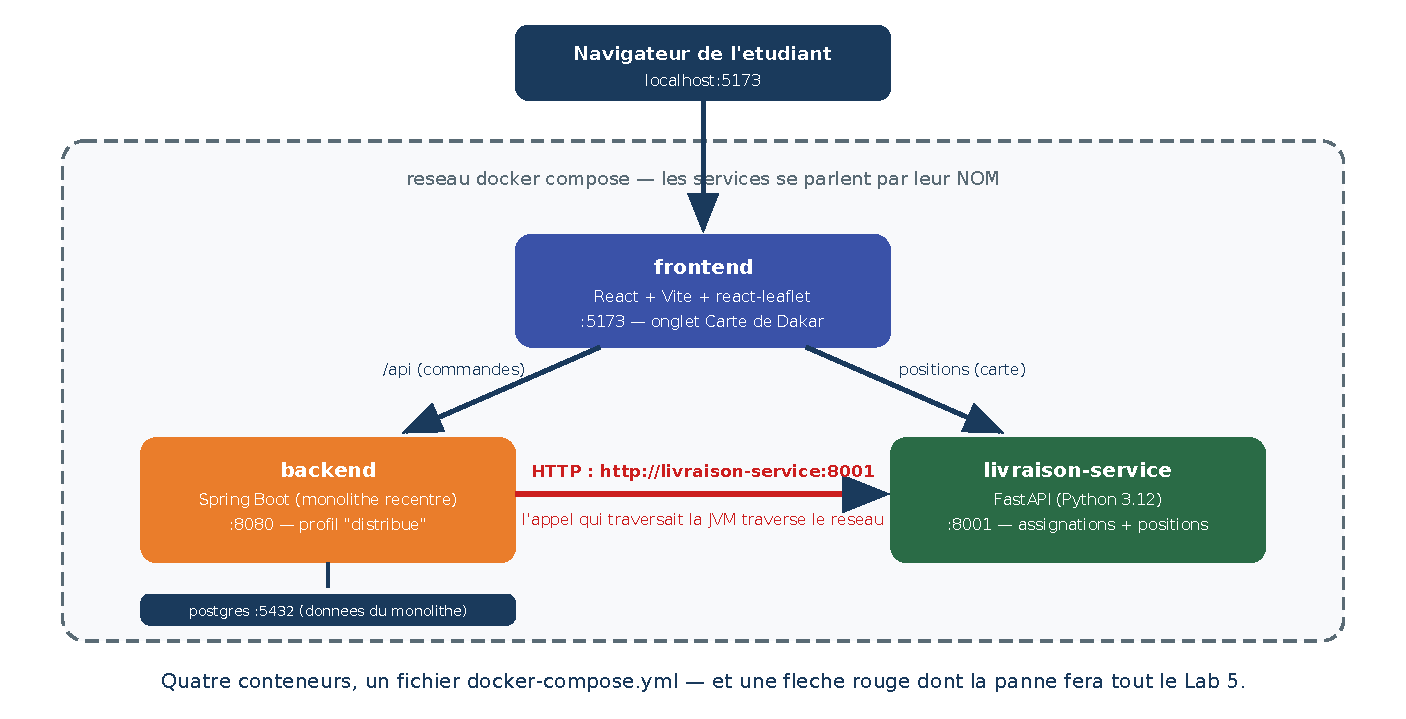
\includegraphics[width=0.80\textwidth]{figs/figK_compose.pdf}
\caption{L'orchestre : le nom du service est son adresse sur le réseau compose.}
\end{figure}

\subsection{La carte de Dakar}

\begin{lstlisting}[language=bash]
cd frontend && npm install react-leaflet leaflet
\end{lstlisting}

Le Rédacteur ajoute l'onglet « Carte » : un composant \texttt{CarteDakar}
centré sur Dakar, les restaurants en marqueurs fixes, et --- pour la
commande sélectionnée --- le livreur en marqueur mobile, dont la position
est interrogée \textbf{directement auprès du service Python} toutes les
3 secondes :

\begin{lstlisting}[language=java]
// Le coeur du composant (extraits -- le squelette complet est fourni
// dans le zip de la seance) :
<MapContainer center={[14.70, -17.45]} zoom={13} style={{height: "480px"}}>
  <TileLayer url="https://{s}.tile.openstreetmap.org/{z}/{x}/{y}.png" />
  {restaurants.map(r => <Marker key={r.id} position={positionDe(r)} />)}
  {positionLivreur && <Marker position={positionLivreur} icon={iconeScooter} />}
</MapContainer>

// Le polling : toutes les 3 s, si une commande CONFIRMEE est suivie
useEffect(() => {
  if (!livreurSuivi) return;
  const minuteur = setInterval(async () => {
    const r = await fetch(`${URL_LIVRAISON}/livreurs/${livreurSuivi}/position`);
    setPositionLivreur(await r.json());
  }, 3000);
  return () => clearInterval(minuteur);
}, [livreurSuivi]);
\end{lstlisting}

Lancez tout : \texttt{docker compose up --build}. Commandez un mafé chez
Aminata, confirmez, ouvrez la carte : \textbf{le scooter d'Ibrahima avance
vers Ouakam}. Cette fonctionnalité entière --- positions, interpolation,
demain le trafic réel --- vit dans le service Python : le bénéfice de
l'extraction, à l'écran.

\begin{exemple}
Deux questions légitimes, deux choix assumés. \emph{« Et l'adresse exacte
du client ? »} --- SénResto travaille à la granularité du \textbf{quartier} :
la distance est calculée (vraie formule de Haversine, vraie vitesse) sur le
trajet \textbf{livreur $\to$ restaurant $\to$ client}, chaque étape au
\emph{centroïde} de son quartier. Une adresse postale exigerait un service
de géocodage externe : hors périmètre, et l'approximation est honnête.
\emph{« Le trajet atteint 100\,\% mais la commande reste EN\_LIVRAISON ? »}
--- Oui : la simulation est visuelle, le changement de statut reste manuel.
Notez l'agacement que cela provoque : \emph{le service sait que la course
est finie...} c'est exactement un événement candidat pour le Lab 5.
\end{exemple}

\begin{warningbox}
\textbf{L'état qui s'évapore --- votre premier vrai problème distribué.}
Les commandes vivent dans PostgreSQL (persistant) ; les courses et
disponibilités vivent \textbf{en mémoire du service Python}. Redémarrez
\texttt{livraison-service} : les courses sont oubliées, tous les livreurs
redeviennent disponibles... alors que la base affirme le contraire. Deux
services, \textbf{deux vérités, aucune synchronisation}. Constatez-le
(redémarrez le service pendant une course), notez-le dans l'ADR --- et
gardez la blessure ouverte : la réconciliation d'état par événements est
un des grands sujets du Lab 5.
\end{warningbox}

\subsection{L'experience finale : la panne}

Au vidéoprojecteur, cérémonieusement :

\begin{lstlisting}[language=bash]
docker compose stop livraison-service
\end{lstlisting}

Puis, depuis le frontend : créez une commande (\textbf{ça marche} --- le
monolithe vit), et tentez de la \textbf{confirmer}. Observez : le 503
après ~2 secondes (votre timeout), le message propre (votre
gestionnaire d'erreurs). Constatez et notez :

\begin{itemize}[nosep]
  \item la mort de \texttt{livraison-service} a \textbf{amputé} la
        confirmation --- couplage \emph{temporel} : les deux doivent être
        vivants \emph{au même instant} ;
  \item et pourtant les SMS, le paiement, eux, n'ont besoin d'aucune
        réponse immédiate... pourquoi devraient-ils dépendre de la
        disponibilité de qui que ce soit ?
\end{itemize}

Redémarrez (\texttt{docker compose start livraison-service}), confirmez :
tout revient. La question reste, ouverte et brûlante --- c'est le Lab 5.

\begin{tagbox}
Compose complet fonctionnel, carte vivante, panne provoquée et documentée :
\begin{center}
\texttt{git tag lab4-final \&\& git push origin lab4-final}
\end{center}
\end{tagbox}

% =====================================================================
\section{Recapitulatif : qui a fait quoi}
% =====================================================================

\begin{center}
\small
\begin{tabular}{p{0.16\textwidth}p{0.26\textwidth}p{0.26\textwidth}p{0.22\textwidth}}
\toprule
\textbf{Rôle} & \textbf{Étape 1} & \textbf{Étape 2} & \textbf{Étape finale} \\
\midrule
Le Doyen & relecture du contrat & invariant \texttt{commandes} intact & la panne au projecteur, ADR \\
\addlinespace
L'Huissier & --- & les deux profils Spring & \texttt{docker-compose.yml} \\
\addlinespace
Le Rédacteur & --- & --- & l'onglet Carte (react-leaflet) \\
\addlinespace
Le Notaire & contrat HTTP vs API module & \texttt{AdaptateurLivraisonHttp} + 503 & vérif. messages d'erreur \\
\addlinespace
L'Appariteur & \texttt{main.py} FastAPI + curl & --- & \texttt{Dockerfile} du service \\
\bottomrule
\end{tabular}
\end{center}

% =====================================================================
\section{L'ADR du jour}
% =====================================================================

L'\textbf{Architecte du jour} signe l'\textbf{ADR n\up{o}4 : « Pourquoi
extraire Livraison --- et pourquoi pas les autres ? »}
(\texttt{docs/adr/adr-004-extraction.md}). Exigence nouvelle : une section
\emph{non-décisions} qui passe les six autres modules en revue et justifie
leur maintien. Alternatives sérieuses : tout garder en modulith (statu quo
défendable !) ; extraire en Java plutôt qu'en Python. Conséquences
négatives à assumer : la latence, la troisième issue, deux stacks à
maintenir, le déploiement qui exige compose.

% =====================================================================
\section{Livrable et criteres de reussite}
% =====================================================================

\begin{center}
\small
\begin{tabular}{p{0.62\textwidth}p{0.28\textwidth}}
\toprule
\textbf{Critère} & \textbf{Vérification} \\
\midrule
Les 4 tags du lab présents & \texttt{git tag} \\
10 juges verts en profil défaut (sans Docker ni Python) & \texttt{./mvnw clean test} \\
Le service répond aux 4 endpoints, 409 compris & \texttt{curl} \\
\texttt{commandes} : zéro ligne modifiée & \texttt{git diff} ciblé \\
Timeouts explicites + 503 traduit & relecture + panne \\
\texttt{docker compose up} : parcours complet, carte vivante & démonstration \\
La panne provoquée, observée, réparée & historique + notes \\
ADR n\up{o}4 avec sa section non-décisions & \texttt{docs/adr/} \\
\bottomrule
\end{tabular}
\end{center}

% =====================================================================
\section{Vers le Lab 5 : ne plus mourir ensemble}
% =====================================================================

Vous avez vu une commande refuser d'être confirmée parce qu'un
\emph{autre} processus était éteint. Pour l'assignation, ce couplage
temporel est presque légitime --- il faut une réponse. Mais les SMS ? Le
paiement ? Informer n'exige pas que le destinataire soit réveillé :
il suffit que le message \textbf{attende quelque part}. Ce quelque part
s'appelle un \emph{broker} --- RabbitMQ --- et au Lab 5, vos événements
du Lab 3 traverseront le réseau par lui : notifications et paiement
deviendront des consommateurs qu'on peut éteindre, rallumer, et qui
rattrapent leur retard sans perdre un seul message. L'apothéose du
semestre. Votre \texttt{lab4-final} en sera le point de départ.

\vspace{1em}
\begin{center}
\textit{Fin du Lab 4 --- Dr. El Hadji Bassirou TOURE --- DMI/FST/UCAD}
\end{center}

\end{document}
